
\documentclass{beamer}
\usepackage{hyperref}
\usepackage{listings}
\usepackage{graphicx}
\usepackage{wasysym}
\usepackage{graphics}
\date{\today}
\lstdefinestyle{basic}{
    captionpos=t,%
    basicstyle=\footnotesize\ttfamily,%
    numberstyle=\tiny,%
    numbers=left,%
    stepnumber=1,%
    frame=single,%
    showspaces=false,%
    showstringspaces=false,%
    showtabs=false,%
    %
    keywordstyle=\color{blue},%
    identifierstyle=,%
    commentstyle=\color{gray},%
    stringstyle=\color{magenta}%
}
\usetheme{Madrid}
\usecolortheme{fly}
\title{Synergia Refactor}
\setbeamertemplate{navigation symbols}{}
\subtitle{Goals, Plans and Status}
\author{James Amundson}
\date{September 23, 2010}

\begin{document}


\frame{\titlepage}


\defverbatim[colored]\fckdplljecneiikediijkggeidikjagm{
\begin{lstlisting}
lattice = Mad8_reader().get_lattice("fodo", "fodo.lat")
#space_charge = Space_charge_3d_open_hockney(grid)
space_charge = Collective_operator("space charge")
lattice_simulator = Lattice_simulator(lattice, map_order)
stepper = Split_operator_stepper(lattice_simulator, space_charge,
                                          num_steps)
bunch = generate_matched_bunch_transverse(lattice_simulator, emit, emit, stdz, dpop,
                                        num_real_particles, num_macro_particles,
                                        seed=seed)
diagnostics_writer_step = Diagnostics_writer("example_full2.h5", Diagnostics_full2())
diagnostics_writer_turn = Diagnostics_writer("example_particles.h5",
                                                  Diagnostics_particles())
propagator = Propagator(stepper)
propagator.propagate(bunch, num_turns, diagnostics_writer_step, diagnostics_writer_turn)
\end{lstlisting}
}
\defverbatim[colored]\jicaagjlckagohejccdkdbaimoobcfgd{
\begin{lstlisting}
components/test_example.py
\end{lstlisting}
}



\section{Background}


\begin{frame}
 \frametitle{Background}
  

\begin{columns}
\column{0.5\textwidth}
\begin{itemize}
  \item Synergia1 was a combination of IMPACT (F90) + CHEF (C++) + frontend (Python)
\begin{itemize}
  \item IMPACT provided the driver
\end{itemize}
  \item Synergia2 started as a proof-of-concept for a Python driver
\begin{itemize}
  \item Design heavily influenced by IMPACT and Forthon
\end{itemize}
  \item Synergia2 has evolved from there
  \item Synergia2 evolved its own C++ space charge solvers
\begin{itemize}
  \item IMPACT solvers have atrophied
\end{itemize}
  \item Evolution is not always pretty
\end{itemize}
\column{0.5\textwidth}
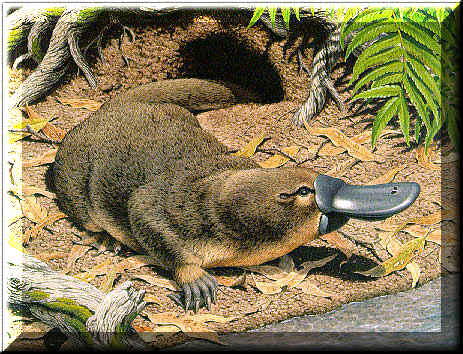
\includegraphics[width=\textwidth]{Platypus.jpg}
\end{columns}

  
 \end{frame}

\section{Goals}


\begin{frame}
 \frametitle{Synergia Goals}
  

\begin{itemize}
  \item World domination
\begin{itemize}
  \item Include all collective effects in beam dynamics
  \item Greatly expand user base
\end{itemize}
\end{itemize}

  
 \end{frame}
\begin{frame}
 \frametitle{Refactor Goals}
  

\begin{itemize}
  \item Make code more usable, extensible, maintainable and robust
\begin{itemize}
  \item also, more apple pie
\end{itemize}
  \item Implement a clean Python/C++ separation
\begin{itemize}
  \item Pure C++ objects
  \item Pure Python objects
\end{itemize}
  \item Internal cleanup
\begin{itemize}
  \item No MPI COMM WORLD, single multi-dimensional array implementation, etc.
\end{itemize}
  \item Rigorous testing
  \item Create a stable API
  \item End-user documentation
  \item Create abstractions for common modifications
\begin{itemize}
  \item Previously done on-the-fly
\end{itemize}
\end{itemize}

  
 \end{frame}

\section{Refactor Plans}


\begin{frame}
 \frametitle{Refactor Features}
  

\begin{itemize}
  \item Standalone C++ programs now possible
\begin{itemize}
  \item Not practical for everyday simulations
\begin{itemize}
  \item Except as a last resort
\end{itemize}
  \item Useful for benchmarking, optimization
\end{itemize}
  \item Extensive unit tests
  \item Documentation (using Sphinx and Doxygen) part of build system
\end{itemize}

  
 \end{frame}

\section{Refactor Status}


\begin{frame}
 \frametitle{Refactor Status}
  

\begin{itemize}
  \item Fermilab CPA group has completed (or about to complete) several simulation deadlines
\begin{itemize}
  \item Will work more on code during next few months
\end{itemize}
  \item Single-particle portion of code working
\begin{itemize}
  \item Has unit tests
  \item Not yet implemented: ramping, apertures
\end{itemize}
  \item Proof-of-principle documentation working
\begin{itemize}
  \item \url{http://home.fnal.gov/~amundson/synergia-refactor/index.html}
\end{itemize}
\end{itemize}

  
 \end{frame}
\begin{frame}
 \frametitle{Code Statistics}
  

\begin{columns}
\column{0.5\textwidth}
\includegraphics[width=\textwidth]{language_breakdown.png}
\column{0.5\textwidth}
\includegraphics[width=\textwidth]{test_breakdown}
\end{columns}

  
 \end{frame}
\begin{frame}[shrink=42]
 \frametitle{Prototype Application}
  



\fckdplljecneiikediijkggeidikjagm



\emph{The above code snippet contains all the important code. The entire working application can be found in}

\jicaagjlckagohejccdkdbaimoobcfgd



  
 \end{frame}


\end{document}

